\section[EVOLUTIONARY DUNGEON DESIGNER]{EVOLUTIONARY DUNGEON \\DESIGNER}
\label{sec:edd}
This section presents the~\acrfull{edd} research tool, all its subsystems and features, and the multiple interactions between the human designer and the computational designer. First, it describes the tool's objectives, the iterations it has gone through, and game design patterns as a significant feature. Then, it presents and discusses the room and narrative generation process, the intertwined attempts, and multiple designer interactions. Finally, it describes the tool's workflow and presents some examples.

% \begin{itemize}
%     \item Total description of EDD, and what it enables
%     \item workflow and development
% \end{itemize}

\begin{figure}[!h]
\centerline{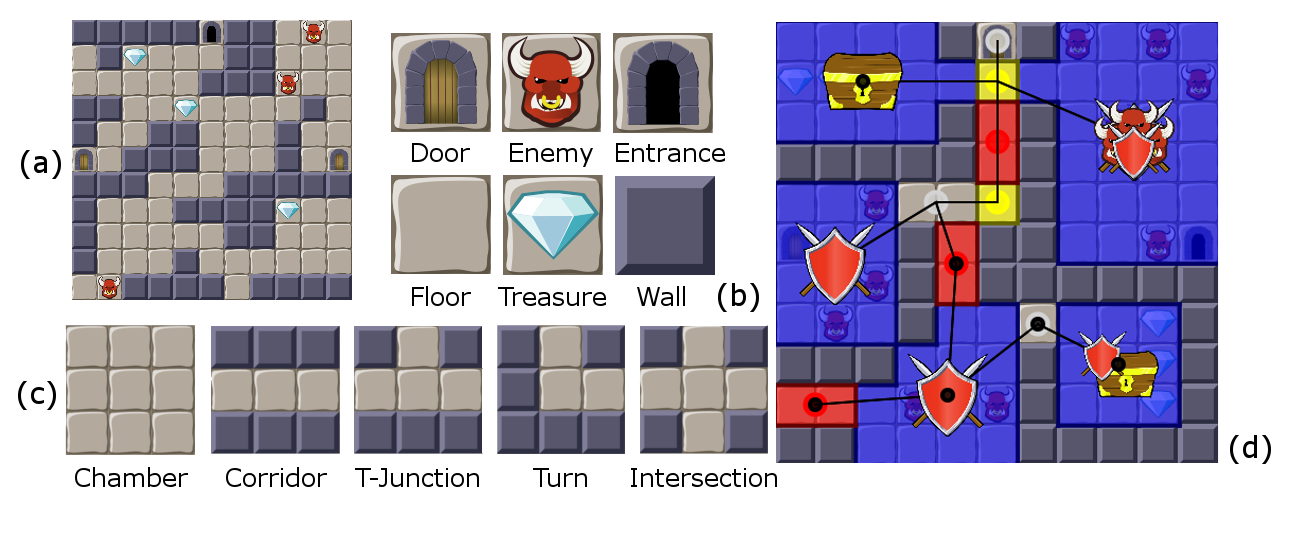
\includegraphics[width=\textwidth]{figures/EDD-figs/map-figure.png}}
\caption{Main level design components in EDD. (a) Basic example room, (b) different placeable tiles (the boss tile looks the same as the enemy tile but 3 times bigger), (c) spatial-patterns and (d) meso-patterns} \label{fig:tilesPats}
\end{figure}

The~\acrshort{edd} is an~\acrshort{micc} system to create adventure and dungeon crawler content, similar to the ones found in Zelda~\cite{tloz} or the Binding of Isaac~\cite{bindingISAAC}. The main feature of~\acrshort{edd} is the collaboration between human and computational designer to create levels and narrative. Within level design, the human designer focuses on editing the room to design their goals while in parallel, they are continuously offered a set of suggestions adapted to their current design. In addition, the designer's design is continuously evaluated for design patterns, feasibility and playability constraints, and enhanced information of the rooms such as door safety or enemy-treasure balance. Within narrative design, the human designer can focus on the creation of quests and overarching narrative structures, while the computational designer collaborates by suggesting quest actions and auto-completing quests, and suggesting diverse narrative structures adapted from the designers structure and level design constraints. Likewise, the computational designer assesses the level design changes that might invalidate quests and change narrative structure constraint.

% the designer is provided with additional information

The first iteration of~\acrshort{edd} was described and presented by Baldwin et al.~\cite{baldwin_mixed-initiative_2017,baldwin_towards_2017}. In their work, the aim was on creating the first steps towards a~\acrshort{micc} system that allowed the designer to create fixed-sized individual rooms while receiving four generated rooms with diverse targets upon request.~\acrshort{edd} was developed further with a revamped UI, allowing the creation of complete dungeons, and providing augmented information on the suggestions compared to the current design~\cite{alvarez_fostering_2018,alvarez_assessing_2018}. The next version of~\acrshort{edd} allows the designer to create dungeons in whatever layout preferred, and incorporates the~\acrlong{icmape}, providing a customizable grid of suggestions steered by the selected feature dimensions~\cite{alvarez_empowering_2019,alvarez_interactive_2020}. Narrative aspects were included in the following iterations. Automatic objective assessment~\cite{flodhag_make_2020} and quest creation and generation~\cite{alvarez_questgram_2021,larsson_queststories_2021} were included in the next iteration. Dungeons were assessed for overarching objective placement, and designers could add different NPCs and quest items in their levels to couple quest actions to them, receiving suggestions from the computational designer. Finally, the last iteration included the creation of overarching narrative structures~\cite{alvarez_tropetwist_2022,alvarez_story_2022}, where designers could set characters, factions, conflicts, objectives, and main or side events, while receiving suggestions in the same line as when creating rooms using the~\acrshort{icmape}. All of the available views where the designer can create content and interact with different parts of the system are shown in figure~\ref{fig:eddWorkflow}. In addition,~\acrshort{edd} now includes prototype implementations of different designer models: the designer preference model~\cite{alvarez_exploring_2020} and designer personas~\cite{alvarez_designer_2022}.

\begin{figure}[t]
\centerline{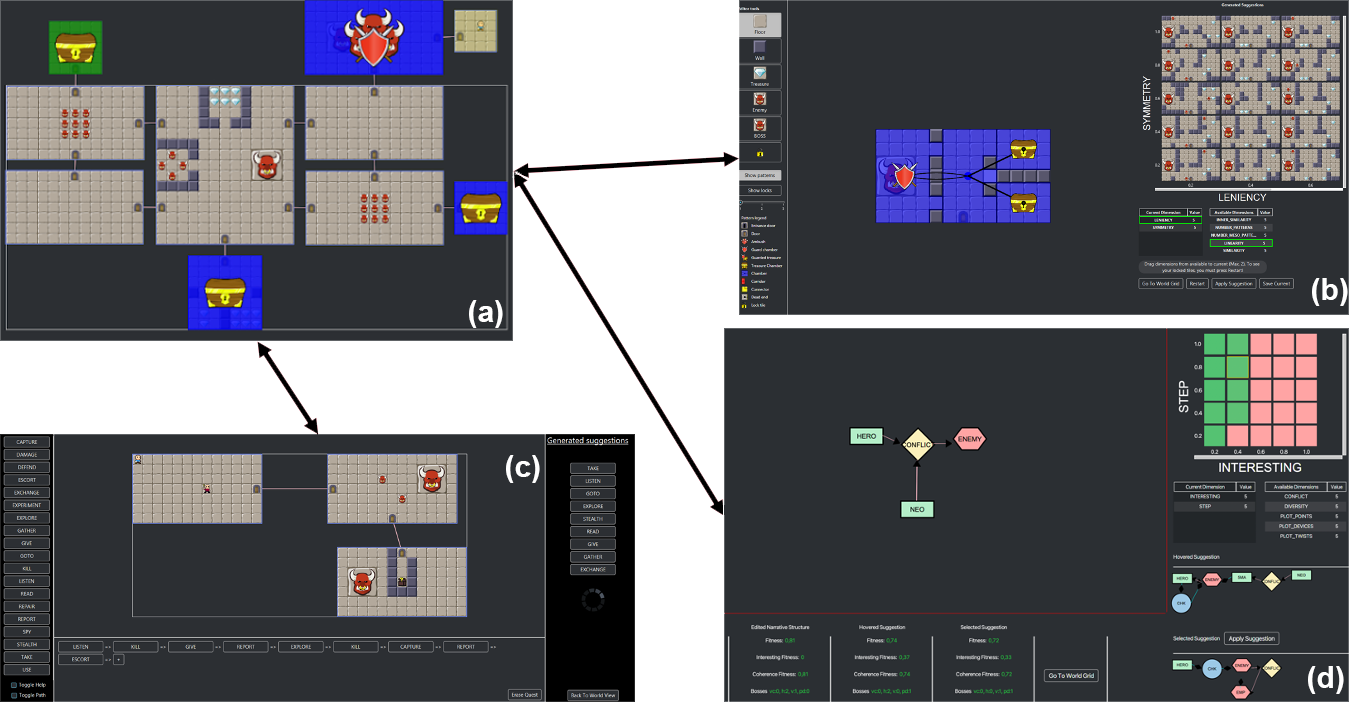
\includegraphics[width=\textwidth]{figures/EDD-figs/eddworkflow.png}}
\caption{Workflow of the~\acrlong{edd}. (a) Shows the world view with a prototype dungeon (\textsc{papers i, ii, iii}) and it's automatically assessed objectives (\textsc{paper vi}). (b) Shows the room view, the main interactive view of~\acrshort{edd}. In this view the designer can edit their room while the computational designer is offering suggestions for their design (\textsc{papers i, ii, iii, v}). (c) Shows the QuestGram view, where designers can use their current dungeon to add different quest actions linked to the room elements (\textsc{paper vii}). Finally, (d) shows the Story Designer view, where designers can create the overarching narrative structure for their game (\textsc{papers x, xi}).} \label{fig:eddWorkflow}
\end{figure}

%Finally, the latest version of~\acrshort{edd} is the one presented on this thesis, which incorporates the~\acrshort{icmape} and allows the designer to create dungeons in whatever layout preferred~\cite{alvarez_empowering_2019,alvarez_interactive_2020}. In addition,~\acrshort{edd} now includes prototype implementations of different designer models: the designer preference model~\cite{alvarez_exploring_2020} and designer personas~\cite{alvarez_designer_2022}.




% ~\acrshort{edd} has four views that enable the~\acrshort{micc} wokflow.

% \subsection{Room Configuration}
\subsection{Level Design}

Dungeons in~\acrshort{edd} are a cyclical graph composed of interconnected rooms. Rooms are a rectangular $M \times N$ grid of tiles, which might be: \emph{Floor}, \emph{Wall}, \emph{Treasure}, \emph{Enemy}, \emph{Enemy Boss}, and \emph{Door} (all shown in figure~\ref{fig:tilesPats}.b). \emph{Wall} tiles are obstacles that cannot be traversed by the player, while all the other are considered passable and could be ``interacted'' by the player. \emph{Enemy boss} tiles are a special type of tile that occupies a $3\times3$ area, as its challenge might be comparable to nine enemies, and only two at a time can co-exist in a room. Doors cannot be placed at will by the designer but might be added when connecting rooms in the world view. 

%\subsubsection{Level Design Patterns}

An essential part of~\acrshort{edd} is its use of level design patterns to hierarchically divide a room into micro-patterns (inventorial and spatial patterns) and their combination into meso-patterns. The level design patterns in~\acrshort{edd} are based on~\cite{bjork_patterns_2004,dahlskog_patterns_2015,dahlskog_procedural_2014}. While~\acrshort{edd} is an~\acrshort{micc} tool to create dungeons for adventure games, we can leverage design patterns to create a generic and domain-independent tool. Through this, we do not need strict definitions or constraints based on specific tiles or functionalities. Rather we rely on patterns that can be made into specific content by the designer if needed.

The design patterns are used in two ways. First, they are used to evaluate the designer's design and show the designer how the system categorizes different parts of the rooms. Second, and more important, design patterns are used to estimate the quality of a generated room. By extracting the patterns of the designer's design and evaluating the generated rooms based on that, design patterns can be used as goals to be achieved by the generated content. In EDD, we have defined \emph{micro-patterns} as the minimum bits that compose the room, and are divided into \emph{inventorial} and \emph{spatial} patterns. \emph{Inventorial patterns} are individual passable tiles, and \emph{spatial patterns}, are a combination of passable tiles and walls resulting in chambers, corridors, and different intersections. 

\emph{Meso-patterns} are the next level in the design pattern hierarchy. They are the composition of micro- and meso-patterns. The meso-patterns that are currently implemented are (shown in figure~\ref{fig:tilesPats}.d): \emph{dead-end}, \emph{ambush}, \emph{guard chamber}, \emph{treasure chamber}, \emph{guarded treasure}.

%To perform this evaluation, design patterns in~\acrshort{edd} calculate a \emph{quality} metric. For instance, the enemy pattern's quality is a combination of the number of enemies placed in the room and how they are distributed. Thus, if the enemies are a certain amount and are not simply added next to each other but distributed with other patterns, the ``enemy quality'' improves.



%the work by Bjork and Holopainen~\cite{bjork_patterns_2004}, Dahlskog et al.~\cite{dahlskog_patterns_2015}, and Dahlskog and Togelius~\cite{dahlskog_procedural_2014}. While~\acrshort{edd} is~\acrshort{micc} tool to create dungeons for adventure games, we can leverage design patterns to create a generic and domain-independent tool. Through this, we do not need strict definitions or constraints based on specific tiles or functionalities. Rather we rely on patterns that can be made into specific content by the designer if needed.

% without strict definitions or constraints based on specific tiles or




% Through this, the system extract the patterns composing the rooms and use it as an estimator of 

% which allows for the comparison of an objective estimation, and to extract possible .

% and through combining these patterns form a new set of patterns. Design patterns are inspired 
% Design patterns 

% \paragraph{Tiles}

% Further, the designer can edit all the rooms with the following set of tiles: \emph{Floor}, \emph{Wall}, \emph{Treasure}, \emph{Enemy}, and \emph{Boss}. When editing their rooms, the designer can activate

% \paragraph{Micro-patterns}

% Micro-patterns are the minimum bits that compose an artifact, in this case, a room. Micro-patterns in~\acrshort{edd} are divided into inventorial patterns and spatial patterns. Inventorial patterns relate to each individual passable tile; thus, each passable tile is represented by an inventorial pattern, and its aggregated quality can be measured. Spatial patterns are composite patterns based on the used space and are a combination of passable and unpassable tiles (i.e., walls).

% Inventorial patterns relate to passable tiles. Yet, rather than calculating each pattern's quality based on individual tiles, they are calculated as a whole. For instance, two enemies placed in different parts of the level will have a shared quality. Inventorial patterns' quality is a trivial calculation based on a user-defined target proportion and the number of tiles of the same type in the room. Doors are a special inventorial pattern, where their quality is based on a linear combination of four measures: \emph{door safety}, \emph{door greed}, \emph{average treasure safety}, and \emph{treasure safety variance}.

% Spatial patterns focus on each room's spatial characteristics and are categorized as a combination of passable tiles and walls. A combination of spatial patterns might give an indication of the type of gameplay the designer wants to create. For instance, multiple interconnected chambers in a room could indicate more small goals within a room and where combat could take place with more maneuvers.

% The spatial patterns are (shown in figure~\ref{fig:tilesPats}.c): \emph{chamber}, \emph{corridor}, \emph{t-junction}, \emph{turn}, and \emph{intersection}. Like inventorial patterns, they are also driven by user-defined targets for creating ``high-quality'' areas and user-defined minimums for areas to be identified as a spatial pattern. For instance, a chamber is identified if there exists at least a $3 \times 3$ open area in a room. Quality is also a trivial calculation based on the expected user-defined targets and the spatial pattern's actual proportion.
% % In figure~\ref{fig:tilesPats}.b, all the possible spatial patterns are shown, and these ar. 

% % Nevertheless, when both inventorial and spatial patterns are used to evaluate generated rooms while the designer works in their design, the user-defined targets are replaced, to a large extent, by the designer's design.
 
% \paragraph{Meso-patterns}

% Meso-patterns are the next level in the design pattern hierarchy. They are identified as pattern compositions and are defined as how micro- and meso-patterns relate. For instance, a chamber (spatial pattern) containing some enemies (inventorial patterns) would result in a ``guarded chamber'' meso-pattern.

% The meso-patterns that are currently implemented are (shown in figure~\ref{fig:tilesPats}.d): \emph{dead-end}, \emph{ambush}, \emph{guard chamber}, \emph{treasure chamber}, \emph{guarded treasure}. \emph{Dead-end} is the only meso-pattern that acts as a pattern modifier rather than a composition of patterns. They are calculated by traversing the pattern graph from all the spatial patterns containing a door to all the other spatial patterns. If any spatial pattern can only be reached by one way, the spatial pattern and all the steps towards it that are not connected to other patterns are classified as dead-ends. For the rest of the meso-patterns, the crucial aspect is that their main component is a chamber (spatial pattern). Thus, these meso-patterns can be seen as a specialization of the chamber. 

% \textbf{Ambush:} Relates to a chamber containing at least one enemy and a door (inventorial pattern). Similar to others, the amount of enemies is also a user-defined minimum. 

% \textbf{Guard chamber}: Relates to a chamber containing at least two enemies (inventorial pattern) and nothing else. Similar to others, the amount of enemies is also a user-defined minimum. 

% \textbf{Treasure chamber:} Relates to a chamber containing at least two treasures (inventorial pattern) and nothing else. Similar to others, the amount of treasures is also a user-defined minimum. 

% \textbf{Guarded treasure}: Relates to a chamber, which is a dead-end, containing at least two treasures (inventorial pattern) and nothing else, but preceded by a guarded chamber. Similar to others, the amount of treasures is also a user-defined minimum. 





% \subsubsection{Macro-patterns}

\subsubsection{Room Generation}

The main feature of~\acrshort{edd} is to suggest variations of the designer's work that are adapted to their design, interesting, and can foster the designer's creativity. Through this, we seek that~\acrshort{edd} ends representing the role of a colleague, as discussed by Lubart~\cite{lubart_how_2005}. The suggestions use the designer's current room configuration as target ratios (e.g., the number of corridors, the number of inventorial patterns, etc.) to provide adaptive suggestions. However, due to the algorithm's nature, the designer is also suggested content that respects these ratios but might use them differently with a different goal.

For instance, if the designer is creating a room with many corridors, such as a labyrinth, they will be provided with suggestions with a similar distribution of corridors, but utilizing the rest of space in different ways, as shown in figure~\ref{fig:corridorExample}.

\acrshort{edd} uses the~\acrshort{icmape} (explained in detail in~\textsc{papers III, V}) to generate and suggest rooms to the designer. Its main features are the use of divergent and convergent searches, the search space division into cells, the use of behavior feature dimensions, the constrained population per cell, and the designer's ability to interact with it. Through this process,~\acrshort{edd} can provide a grid of evolved high-performing suggestions, adapted to the designer's current design, while representing a diverse set of solutions. For instance, in figure~\ref{fig:corridorExample}, it is shown multiple evolutionary runs when using the same design and the set of generated suggestions. It can be observed that the designer is provided with a set of suggestions that retained their expected ratios and design, but diverse enough that the designer can browse many different variations. It can also be observed the effect of the different feature dimensions, as some of them do not match the expected ratios adequately. Thus, producing bigger variations in the solutions to explore the search space. In figure~\ref{fig:interactiveMAPE}, it is presented an overview of the~\acrshort{icmape} steps applied to the level design facet and the multiple areas designers can interact.


\begin{figure}[!h]
    \centering
     \subfloat[Example room]{%
       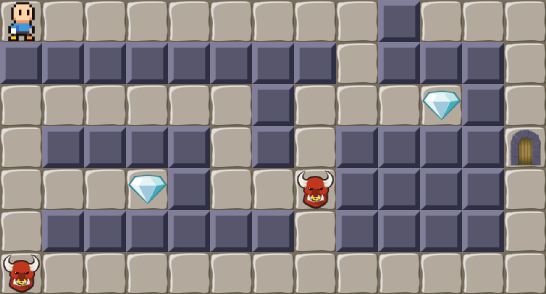
\includegraphics[width=0.48\textwidth]{figures/EDD-figs/corridor_example/currentRoom.png}
     }
     \hfill
     \subfloat[Design Patterns]{%
       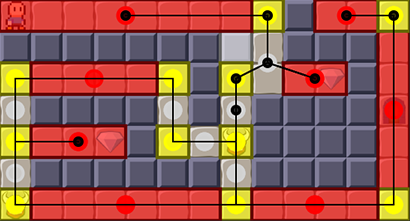
\includegraphics[width=0.48\textwidth]{figures/EDD-figs/corridor_example/room-corridors-final.png}
     }
     
      \subfloat[Meso-pattern and Leniency]{%
       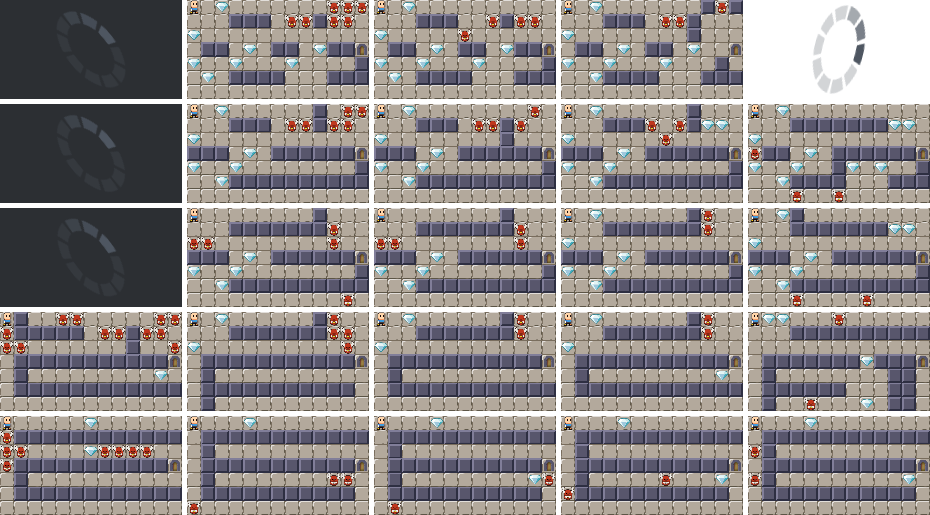
\includegraphics[width=0.48\textwidth]{figures/EDD-figs/corridor_example/meso-leniency-final.png}
     }
     \hfill
     \subfloat[Symmetry and Leniency]{%
       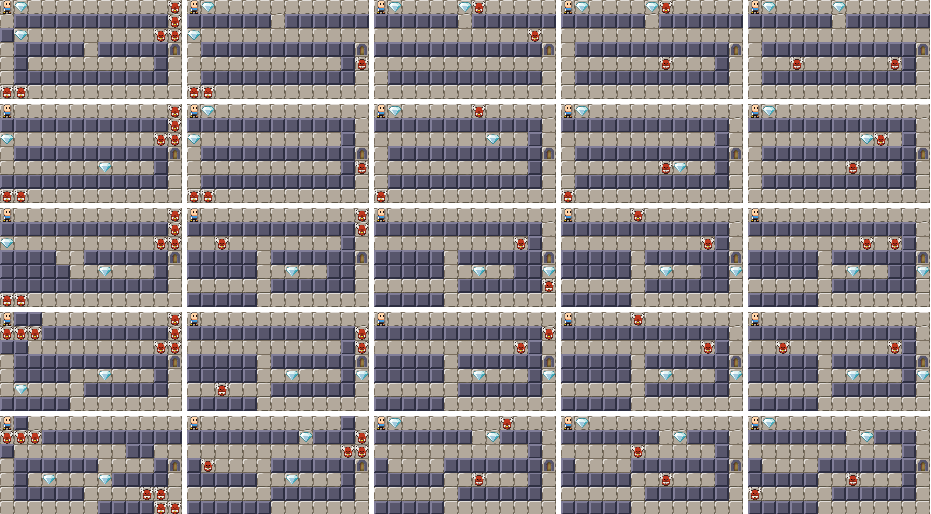
\includegraphics[width=0.48\textwidth]{figures/EDD-figs/corridor_example/sym-leniency-final.png}
     }
    
    \caption{Example of a possible room created by a designer (a), the design patterns identified by the system (b), and two suggestion grids presented to the designer (c and d). The rooms in both suggestion grids, were generated using~\acrshort{icmape} using respectively, \#meso-patterns and leniency (c), and symmetry and leniency (d) as dimensions.}
    \label{fig:corridorExample}
\end{figure}


%\paragraph{Evolutionary Components}

%\acrshort{icmape} is an extension of the Constrained~\acrshort{mape}, which uses a~\acrshort{fi2pop} and~\acrshort{mape} at its core. In our implementation of~\acrshort{icmape}, a solution is deemed infeasible if the playability constraints are not satisfied, i.e., there is a passable tile that is not reachable from at least one door. If this happens, the solution is placed in the respective infeasible population to evolve into a feasible one encouraging diversity in the population.

%Moreover,~\acrshort{edd} implements seven behavior feature dimensions (shown in table~\ref{table:mape-dimensions}). The designer can select one at a time, and only two dimensions can be active at any given time, in order to be able to present the suggestions intuitively to the designer and to focus the search on the pair of dimensions. By giving the designer this interaction, they can effectively reshape the search space of the~\acrshort{icmape}.

%Furthermore, besides using feature dimensions to encounter diverse solutions,~\acrshort{edd} uses a single-objective fitness function to calculate the generated rooms' fitness. The fitness is a weighted sum divided equally between (1) the inventorial aspect of the rooms, which relates to the placement of enemies and treasures in relation to doors and target ratios, and (2) the spatial distribution of the design patterns, which refers to the distribution between corridors and rooms, and the meso-patterns that those encompass. The fitness adapts to the user's current design, automatically informing target ratios and distributions to be achieved by the~\acrshort{ea}.

%The fitness function is shown in Eq.~\ref{fitness_func}. $f_{inventorial}$ is the evaluation of the aggregated and normalized quality of treasures, enemies, and doors (inventorial patterns). Quality refers to positioning, safety, and the relation between inventorial patterns. $f_{spatial}$ refers to the quality and distribution of chambers, i.e. open areas in the room and corridors, and the meso-patterns created within chambers. 

%\begin{equation} 
%\label{fitness_func}
%f_{fitness}(r) = \frac{1}{2}f_{inventorial}(r) \,+ \, \frac{1}{2}f_{spatial}(r)
%\end{equation}


% Cells are first created based on the dimensions selected by the user and proceed to initialize the population based on the user's design, evaluate it and assign each individual to the corresponding cell. Before starting each generation, we check if the dimensions have changed, and if so, recreate the cells and populate them with the previous individuals, and proceed through the evolutionary components. We first select uniformly random which cell to choose parents from, and then we select 5 parents through tournament-selection. Offspring are produced through a two-point uniform crossover operation with a 30\% chance of mutation. Offspring are placed in the correct cell and population after calculating their fitness and dimension's information. Finally, cells eliminate the low-performing individuals that over-cap their maximum capacity. Since interbreeding is not allowed, and can only happen indirectly (i.e. the offspring changing population and then used for breeding in consequent generations), the strategies are repeated for each of the populations.

% This procedure is repeated until the user decides to stop the algorithm. Meanwhile, the EA runs for $n$ generations, and once it reaches the specified limit, it broadcasts the found elites. In order to foster the exploration, we first mutate all the individuals from all the populations and cells (while retaining the previous population), and add them into the same pool together with the current edited room without changes. Finally, we evaluate and assign all the individuals to the correct cells, and cells that are over maximum capacity eliminates low-performing individuals.

% Selection is through competition, 

% That means that with a single run,~\acrshort{icmape} is able to generate a grid of solutions


% aligned to their and are interesting 

% The main feature of~\acrshort{edd} is the computational designer, which main task is to represent the role of a colleague as discussed by Lubart~\cite{LUBART2005-computerPartners}. In order to do this, 

% The formula for calculating the fitness score is the following: 

\subsection{Narrative Design}

Within~\acrshort{edd}, narrative is explored in three individual components: main and secondary objectives based on dungeon's topology and level design patterns (\textsc{paper vi}), quests based on the individual tiles (\textsc{paper vii}), and overarching narrative structure (\textsc{papers x, xi}). These components part from the same idea, using and leveraging patterns and structures to formalize the generation and propose content to the designer. It is important to also highlight that in~\acrshort{edd}, in its current state, these narrative components are subordinate to the level design facet. This means that changes in the rooms and dungeon have effects in the narrative, which the computational designer assess, informs the user of the needed changes, and aids on these changes.

% These narrative components are in relation to the designed dungeon.

%All the narrative components are explored in relation to the designed dungeon. In its current state,~\acrshort{edd} narrative components are effectively subordinate to the level design aspect. This means that changes in the rooms and dungeon have consequences in the narrative, which the computational designer assess, informs the user of the needed changes, and aids on these changes.  

\subsubsection{Automatic Objective Assessment}

Leveraging on the dungeon's structure and the patterns that arise from the designers' design for each level, we calculate possible objectives in the dungeon. The main idea is to utilize the dungeon as much as possible, which means that dead-end rooms without bosses would yield side objectives for players to encourage exploration through side objectives. Likewise, depending on the content within rooms, a room would be selected as the main objective for players, prioritizing boss rooms and rooms farthest from the start position. 

The process is simple and asynchronous from the design tasks, but with significant design impact. It gives insight to designers on what type of objectives are assessed based on the rooms they are designing, and the dungeon's topology. However, these objectives just show the assessment done in EDD, but have no functional use. This means that designers could take this objective assessment, agree with it, change the design to achieve other objectives for players, or disregard the assessment. 

%Then designers could change the design to achieve the objectives they prefer for the players.

\subsubsection{Quest Design}

Narrative was further explored by implementing a quest editor for designers to compose quests within~\acrshort{edd}, called QuestGram (in \textsc{paper vii}). QuestGram provides a new view in EDD for designers to concatenate abstract quest actions connected to individual tiles among all the designed rooms to design quests (a long quest sequence with implicit subquests, which was reformulated as explicit subquests in~\cite{larsson_queststories_2021}). The system also makes use of two new tiles, quest item and quest NPC that certain quest actions can be assigned to. For instance, ``Listen'' can only be associated to quest NPCs, while ``Damage'' can be assigned to several tiles. 

QuestGram is a mixed-initiative system within EDD that complements EDD's original purpose as a mixed-initiative system for level design. The computational designer uses grammars (specifically, L-System) to propose suggestions to the designer based on the quest they have created so far. The grammar, quest actions that are provided to the designer, and the type of NPC are adapted from the work by Doran and Parberry~\cite{doran_prototype_2011}, which analyzed quests in four different MMOs, and extracted their common structure. As the designer adds quest actions and connects them to different tiles, the computational designer continuously generate quests using the grammar, and the ones that match the current quest are used to propose the next possible quest action for the designer. The designer can then either use or disregard this suggestions. They can also request a quest action from the system ad hoc at any position of the quest by simply clickling on it.

QuestGram is coupled to the level design facet since it requires rooms to be designed beforehand for quest actions to be connected to some tangible element. This means that editing the rooms by adding or removing elements affect what quest actions can be added, and can also invalidate parts of the quest in case of tile, doors, or room removal. Once the designer is back at the quest view, they are showed the affected quest actions and can either decide to manually replace, remove, or use the suggestion to readjust their quest. 

%It is based on the system 
%The computational designer 
%the original purpose  level design facet
%, and at the same time, implements 
%How quests are designed within the system. From where does it come, and what are the actions meaning (dont extend)

\subsubsection{Narrative Structure Design}

When creating objectives, stories, and narrative in general, we can consider their design in a different abstraction level. Rather than defining specific objectives, creating quests bit by bit, or coupling these elements to actual in-game elements, we can define narrative structurally, which can describe an experience or story with an abstract representation as argued by Barthes~\cite{barthes_introduction_1966} and Szilas~\cite{szilas_idtension_2003}. We can create structures using a set of generic building blocks that when connected together define narrative structures. This, in turn, define generic aspects of a story, leading to the identification of events, roles, and narrative elements, without the need of defining the plot or how they will take place.

In \textsc{paper x}, we introduced \emph{TropeTwist} as a step towards defining and identifying narrative structures in games. TropeTwist uses tropes extracted from TVTropes~\cite{richmond_tv_2004} as building blocks and patterns, which can compose together structures represented as graphs in TropeTwist. To evaluate and analyze these structures, we defined a set of patterns that can arise from the interconnection of tropes: \emph{micro-patterns}, fundamental narrative units in the system such as conflicts, characters, or plot devices; \emph{meso-patterns}, emerging from the combination of micro-patterns and other meso-patterns, they denote spatial, semanctic, and usability relationships within the narrative graph; and \emph{auxiliary patterns}, used to identify structural gaps in the graph. Patterns are evaluated based on their quality, and in turn, these are used to evaluate the structure as a whole syntactically (i.e., coherence and consistency) and semantically.

TropeTwist was implemented within~\acrshort{edd} as a parallel mixed-initiative system called Story Designer (\textsc{paper xi}). Story Designer lets designers create narrative structures in the form of narrative graphs as seen in fig.~\ref{fig:eddWorkflow}.d, using TropeTwist's building blocks while receiving suggestions adapted to their structures. Suggestions are generated using IC MAP-Elites adapted to generate narrative structures by evolving graph grammars (i.e., adding and removing rules, and changing both their left- and right-hand side part of rules). Thus, the designer can freely create their narrative graph and the computational designer proposes a suggestion grid adapted to their graph, akin to the level design facet. 


%generated by the~\acrshort{icmape}, adapted to generate narrative structures. Narrative structures are encoded as graphs, and IC MAP-Elites evolves graph grammars 

%Within~\acrshort{edd}, we implemented TropeTwist 

% tropes that do not contain meaningful narrative information. 



%The final narrative design system implemented 

%What are narrative struxtures? Express this as narrative graphs. What are the narrative structure patterns, and how are they used within the system.

\begin{figure}[!h]
\centerline{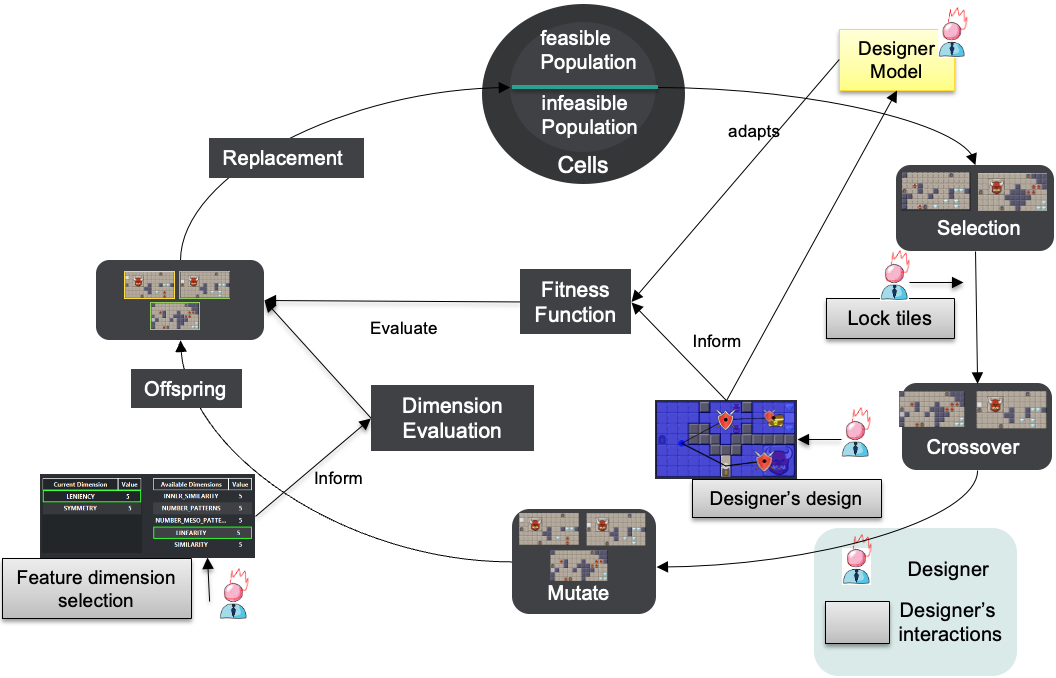
\includegraphics[width=\textwidth]{figures/EDD-figs/all-designers-interactions.png}}
\caption{\acrshort{icmape} evolutionary loop showing the possible designer interactions and what part of the loop these interaction affect} \label{fig:interactiveMAPE}
\end{figure}

\subsection{Designer Interaction}
\label{sec:desInteraction}

A significant feature in~\acrshort{edd}, is the control and interaction designers have with non-intuitive components of the algorithms. In~\acrshort{edd}, the designer always have influence on what the computational designer will create either directly or indirectly. Within the level design facet, the designer can interact with the~\acrshort{icmape} in four different ways: 1) \emph{Locking tiles}: A special tile that locks tiles in the room to be unchangeable (\textsc{paper ii}). 2) \emph{Feature dimensions}: The designer can change the feature dimensions of the~\acrshort{icmape} at any time, reshaping the search space (\textsc{papers iii, v}). 3) \emph{Current design}: The designer is indirectly in constant interaction with the~\acrshort{icmape} by simply designing their room, which adapts the evaluation of generated solutions (\textsc{paper i}). 4) \emph{Designer Model}: As the designer creates their content and uses the suggestions, the system is fed with their interactions, trying to form a model of their preferences (\textsc{paper iv}) and a style and goal model based on their associated designer personas (\textsc{paper ix}).

Within the narrative facet, the designer can interact with it by controlling or influencing the respective algorithm such as the IC MAP-Elites when designing narrative structures or quests, and with the facet itself based on their level design. Concretely, the designer can interact with the algorithms within the facet in two ways: 1) \emph{Developing Quest}: As the designer adds or remove quest actions, the computational designer provides ``next quest action'' suggestions based on the quest up to the selected quest action by the designer (\textsc{paper vii}). 2) \emph{Feature dimensions and narrative structure}: Similar to the level design facet, the designer can interact and change the feature dimensions of the~\acrshort{icmape} when creating narrative structures and at the same time,~\acrshort{icmape} constantly adapts to the designer's narrative structure, leveraging the design as target metric (\textsc{paper xi}). Further, the designer's level design conditions what quest actions will appear and the validity of the quests, what objectives are assessed within the dungeon, and constraints the search space of the~\acrshort{icmape} when generating narrative structures.

% Regarding the indirect control over the narrative facet using the content designed in the level design facet, the designer's design conditions thr


%- Objectives based on their design
% - By adding quest actions, the suggestions take the quest up-to-that point
% - IC MAP-Elites, exactly the same as in level design
% - Their level design conditioning 1) what quest actions will appear and the validity of the quest itself, 2) what objectives are shown, and 3) constraining the search space of IC MAP-Elites when generating narrative structures.

%can interact 


%the designer can interact with the~\acrshort{icmape} in three different ways: 1) \emph{Locking tiles}: A special tile that locks tiles in the room to be unchangeable. 2) \emph{Feature dimensions}: The designer can change the feature dimensions of the~\acrshort{icmape} at any time, reshaping the search space. 3) \emph{Current design}: The designer is indirectly in constant interaction with the~\acrshort{icmape} by simply designing their room, which adapts the evaluation of generated solutions. 

%One of the objectives of this thesis, and a significant feature in~\acrshort{edd}, is the control and interaction designers have with non-intuitive components of the algorithms. In~\acrshort{edd}, the designer can interact with the~\acrshort{icmape} in three different ways: 1) \emph{Locking tiles}: A special tile that locks tiles in the room to be unchangeable. 2) \emph{Feature dimensions}: The designer can change the feature dimensions of the~\acrshort{icmape} at any time, reshaping the search space. 3) \emph{Current design}: The designer is indirectly in constant interaction with the~\acrshort{icmape} by simply designing their room, which adapts the evaluation of generated solutions. 

% The designer can interact with the computational designer, and specifically with the~\acrshort{icmape} that generate the sugthrough

% Besides this, the designer can lock tiles 

% Whenever a designer chooses a suggestion, they are given some extra information 

% \begin{figure}[!h]
% \centerline{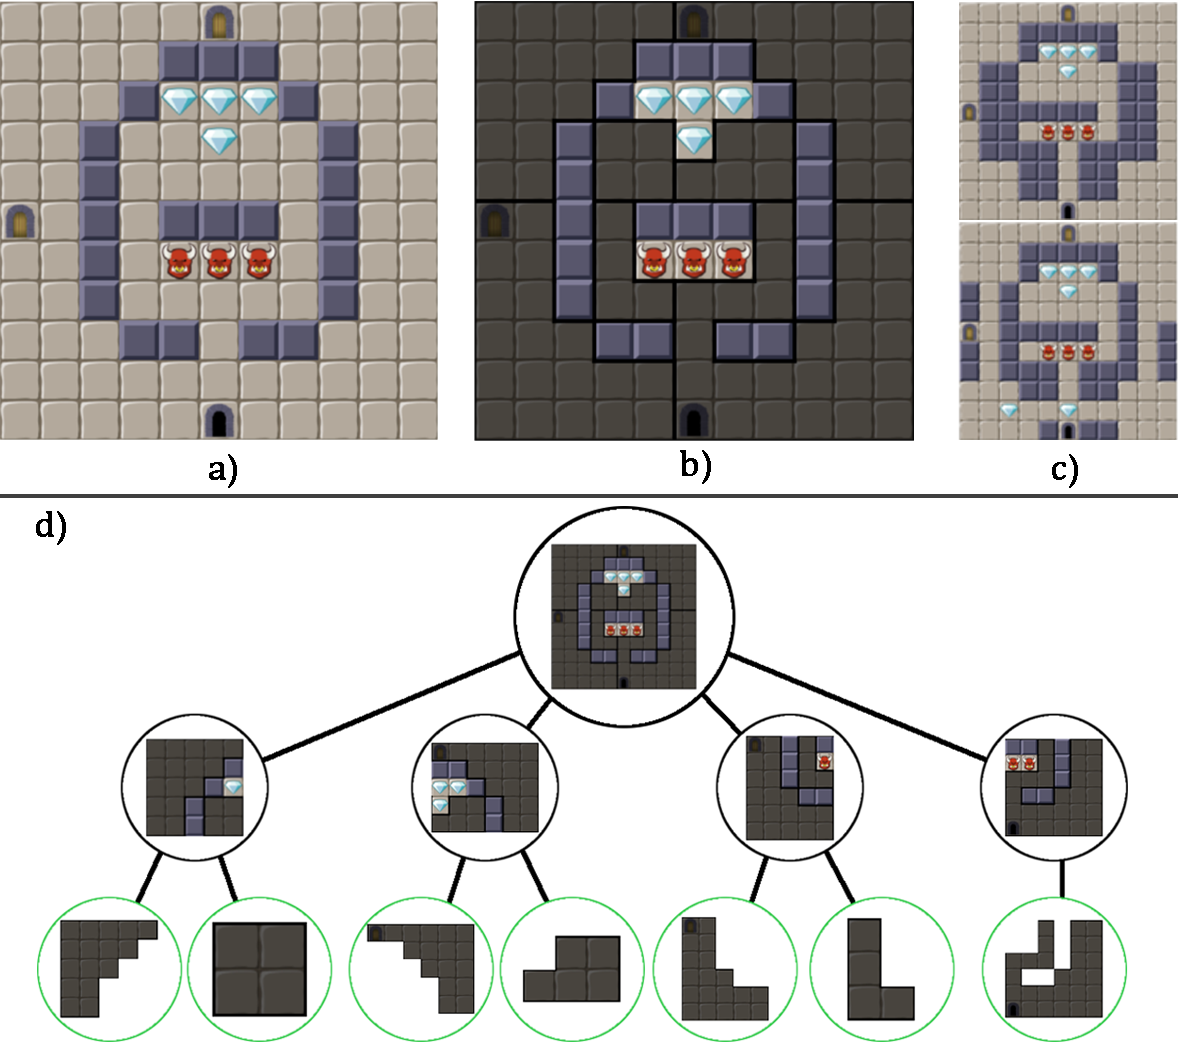
\includegraphics[width=0.8\textwidth]{figures/EDD-figs/map-representation-figure-test.png}}
% \caption{Locking Tiles interaction: (a) A sample edited room with (b) its division into zones based on the tiles locked by the user.(c) Suggestions preserve these locked tiles. (d) The room and its zones are internally represented with a tree structure, where the leaf nodes (green) are the valid genes to apply variation operators.} \label{fig:lockTiles}
% \end{figure}

% \textbf{Locking tiles:} Besides the set of tiles provided to the designer to edit the room, they are given a modifier that allows them to lock tiles in their design, which establishes what tiles or structures must be preserved in the suggestions. By locking tiles, the designer is effectively constraining the building blocks~\acrshort{icmape} have for applying variation operators, as mutation and crossover will only happen on non-locked tiles. However, this also allows~\acrshort{icmape} to focus on the areas that the designer is not interested in, segmenting the room's design and promoting the colleague role. Figure~\ref{fig:lockTiles} shows an example of this interaction and how the genes are segmented in the~\acrshort{ea}.

% % the designer is explicitly interacting with~\acrshort{icmape} by establishing what structures must be preserved in the suggestions.

% \textbf{Feature Dimensions:} A major feature in~\acrshort{icmape} that differentiate the approach to other~\acrshort{mape} variations is the interaction designers have with the algorithm. Feature dimensions are an essential component of~\acrshort{mape}, used to discretizes the behavior space as a grid of cells, illuminating such space. Through this,~\acrshort{mape} can explore the space more vastly by retaining high-performing solutions in cells informed by the feature dimensions encountered in different parts of the behavior space. Furthermore, The designer can interact with these feature dimensions, choosing those of most interest to them. By doing this, the search and solutions encountered are conditioned to the designer's interest. Changing the dimensions reshapes the behavior characteristics where encountered individuals in the search space will be retained.

% \textbf{Current Design:}~\acrshort{edd} uses an adaptive fitness function based on the designer's design by analyzing the room configuration based on the design patterns previously described. This allows the designer to interact indirectly with how~\acrshort{icmape} estimates the quality of the encountered solutions. Therefore, to achieve high-fitness, the generated content will need to have certain similar characteristics than the current design, in order for the content to do not be too disparate from the designer's goal. However, while this might limit the tool's expressivity,~\acrshort{icmape} use of feature dimensions and leverage on convergent and divergent searches still yields diverse solutions.

% Finally, in figure~\ref{fig:interactiveMAPE}, it is presented an overview of the~\acrshort{icmape} steps applied to the level design facet and the multiple areas designers can interact.


% \subsubsection{Designer Modeling}

%\subsection{Workflow}

%\acrshort{edd} has three views that enable the~\acrshort{micc} wokflow depicted in figure~\ref{fig:eddWorkflow}.

%\subsubsection{World View}

%In figure~\ref{fig:eddWorkflow}(a), it is shown the world view. This view provides the designer with an overview of their dungeon while allowing them to create new rooms and edit their connections. The dungeon is a cyclical graph in code, which allows the needed flexibility for the designer to create whatever layout they want. The designer can create or delete any number of rooms and can connect them as needed. By editing these connections, they edit the rooms' entrance and exit doors, effectively changing the layout and gameplay flow. For instance, the designer can create linear gameplay with rooms one after the other, or gameplay that rewards exploration through dead-ends with some side-objective. 

%To edit a room, the designer can: 1) double-click or scroll to zoom-in any room to change the view to the \emph{room view} or 2) select a room and click the ``Suggestions'' button, which will take them to the \emph{suggestion view}

%\subsubsection{Suggestion View}

%In this view (shown in figure~\ref{fig:eddWorkflow}(b)), the designer is proposed six variations to their design based on six different preset room configuration: Favoring open areas, favoring corridors, a mix of open areas and corridors, favoring dead-ends, favoring meso-patterns, and using the actual room configuration. The designer can then go back to the world view or choose any of the suggestions and start editing their room using that as a base in the \emph{room view}.

%\subsubsection{Room View}

%The room view (shown in figure~\ref{fig:eddWorkflow}(c)) is the main view in~\acrshort{edd}, where both the designer and the computational designer interact to co-create rooms. As mentioned above, the designer has five different tiles at their disposal to create a room that fulfills their objective. Besides this, the designer can enable the ``patterns visualization'' that overlays on the designer's design what spatial- and meso-patterns are identified.

%\acrshort{edd} incorporates a feasibility and playability check on the designer's design. This informs the designer if an area in the room is inaccessible from within the room or through another room by adding a red border in their design and an information box. This feasibility check is reused in the~\acrshort{ea} used by the computational designer to generate suggestions for the designer. 

%Moreover, in this view, the designer edits the room as they want, while on the right side of the view, they are suggested a collection of rooms. Whenever a suggestion is selected, a quantitative comparison between the suggestion and the current design is presented to the designer. If the designer decides to replace their design with the suggestion, they apply it and continue the design process. The system aims to give suggestions to the designer that are interesting for them, aligned with their current design, but at the same time different enough to foster their creativity. Designers might not apply any suggestion, but a designer might be interested in doing something similar by observing them. 

%Once the designer finishes editing their room, they can go back to the world view and start another room's design process until they finish their dungeon. 

%\subsubsection{Room Objectives}


%\subsubsection{Quest View}

%\subsubsection{Narrative Structure View}









% These rooms can be examined


% when their design do not fulfill the requirements. These are: 1) there is an area in the room that is inaccessible from within the room or through another room

% As the designer creates their room, the system is constantly 




% In~\acrshort{edd} the designer can create individuals rooms of different sizes and interconnect them to compose dungeons with different types of gameplay. 

